\documentclass{article}

\usepackage[dblblindworkshop]{neurips_2026}
\workshoptitle{Economics for Machine Learning}

\usepackage{microtype}
\usepackage{amsmath,amssymb}
\usepackage{graphicx}
\usepackage{float}
\usepackage{booktabs}
\usepackage{caption}
\usepackage{hyperref}
\usepackage{xcolor}
\usepackage{tikz}
\usepackage{pgfplots}
\pgfplotsset{compat=1.18}
\usepgfplotslibrary{fillbetween}
\usetikzlibrary{shapes,arrows,positioning,calc,backgrounds,fit,patterns,decorations.pathreplacing}

\definecolor{cNYC}{HTML}{0072B2}
\definecolor{cSF}{HTML}{D55E00}
\definecolor{cMUTE}{HTML}{BBBBBB}
\definecolor{cGRN}{HTML}{009E73}
\definecolor{cPNK}{HTML}{CC79A7}
\definecolor{cSKY}{HTML}{56B4E9}
\definecolor{cYEL}{HTML}{E69F00}

\pgfplotsset{
  causalre/.style={
    axis lines*=left,
    tick align=outside, tick pos=left,
    title style={font=\small},
    label style={font=\small},
    tick label style={font=\scriptsize},
    legend style={font=\scriptsize, draw=none, fill=none, row sep=1pt},
    every axis plot/.append style={thick},
  },
  causalre body/.style={ causalre, width=0.42\textwidth, height=3.9cm },
  causalre wide/.style={ causalre, width=0.70\textwidth, height=0.38\textwidth },
}

\hypersetup{colorlinks=true, linkcolor=black, citecolor=black, urlcolor=blue}
\captionsetup{font=small, labelfont=bf}

\renewcommand{\topfraction}{0.92}
\renewcommand{\bottomfraction}{0.85}
\renewcommand{\textfraction}{0.06}
\renewcommand{\floatpagefraction}{0.75}
\setlength{\textfloatsep}{12pt plus 2pt minus 2pt}
\setlength{\intextsep}{2pt plus 1pt minus 1pt}
\setlength{\parskip}{4pt}
\setlength{\abovecaptionskip}{2pt}

\raggedbottom

\title{\bf Absence Is Not Omission:\\
Availability, Vintage, and the Measurement of\\
Selective Benchmark Disclosure}

\author{}
\date{}

\begin{document}
\maketitle

% ---- begin sections/abstract ----
\begin{abstract}
Providers choose which benchmark results a release document prints; independent evaluators score the same models on many more. Dating the instruments seems to answer whether omitted results trail printed ones: a benchmark published after a model shipped could not be reported. The comparison fails as a check on itself. Benchmarks postdating a release trail those predating it by 12.23 percentile points before any label enters, because the date deciding availability also fixes where a model sits in the benchmark's comparison pool, an age-period-cohort collinearity reweighting cannot remove. The failure appears on a leaderboard we did not build: across fourteen HELM Lite releases, fixed models keep identical scores while every win rate moves; a pool-invariant companion moves nothing. Hand-coding every locatable release document, independently second-coded, shows the consequence: the coded gap rejects zero at $+11.4$, yet with labels removed the same releases return $+14.1$, the difference exactly what composition implies. A study built this way turns pool composition into apparent concealment. Reporting is performance-related, reported benchmarks standing 8.7 points above omitted eligible ones within release, yet no possession-grounded test detects withholding, the change-based gap keeping the predicted sign inside its null. Carrying a fixed suite across releases would make later silence informative; adding labels to a moving pool does not.
\end{abstract}
% ---- end sections/abstract ----
% ---- begin sections/intro ----
\section{Introduction}\label{sec:intro}

For each frontier model release, providers disclose benchmark scores through a model card, while third parties execute standardised benchmarks for the same models \citep{liang2022helm,epoch2026hub}. This paper asks whether benchmark availability can identify the older economic question of whether the provider's undisclosed scores are typically worse than their reported scores. Only when the signal is common knowledge does disclosure unravel \citep{grossman1981,milgrom1981}. As \citet{dye1985} details, when receivers cannot distinguish between senders who have no information, and senders who have bad information, receivers treat senders as the same, encouraging withholding. This indistinguishability extends to any research that attempts to analyse what was withheld, since we rely on the endowment, the signal a sender had at time of writing, which we do not observe in the work below.

The presence of benchmark release dates gives a rare ability to bound the endowment exogenously: when benchmarks are never shared before publication, any benchmark released after the model release is necessarily not in the provider's endowment, regardless of whether providers ran it themselves. This lets us distinguish what was able to be disclosed, from what was unable to be disclosed.

First, we provide a new longitudinal study of benchmark disclosure that uses the boundary to construct a panel of a fixed snapshot of an independent benchmarking hub containing 819 model-versions, which we aggregate over scaffold variants to a panel of 353 provider releases, 46 organisations, 74 benchmarks, and 3,082 model-benchmark scores. We provide a verified release date for each benchmark, creating a new panel of 2,355 eligible model-benchmark scores, and 476 ineligible model-benchmark scores.

Second, we show that while the ability to bound the endowment is a unique and powerful feature to understand withholding, constructing a relative ranking of performance is required to judge withholding. Our central analysis compares reported, versus omitted benchmarks that were able to be reported, and requires the relative ranking to be unbiased across the two sides of availability. Instead, there is a 12.23 percentile point difference on average in performance between benchmarks created before the model release, versus those that were created after the model release, with pre-release benchmarks outperforming post-release benchmarks in 78.1\% of the 146 releases that have cells in both groups. None of this calculation uses whether the provider reported the benchmark, and the least biased estimate of the relative ranking remains at 9.14 points. This remains a structural problem, as the verification of the endowment uses the same signal, the release date, that biases our relative ranking \citep{heckman1979}. In economic terms, the presence of benchmark vintages is a free signal to verify the endowment, which \citet{dye1985} demonstrates cannot be known to receivers in general. However, the signal to verify the endowment is not excludable in the relative ranking, and therefore is self-contaminating. This raises a fundamental design challenge for any research that verifies the presence of information via vintage, but then prices evidence using a relative ranking, win rate, or percentile. Not only must reporting decisions be observable, but also the relative ranking must maintain a consistent reference group that is invariant to the endowment.

In our third finding, we extend these concerns beyond our panel. In a sample of 14 published releases for HELM Lite, the pool expands ($30 \to 91$ models); 24 models keep bit-for-bit identical scores; and all their published headline values change (five pairs reversing order). These changes do not show up in a parallel leaderboard maintained by the same group of authors, which presents an absolute headline.
of HELM Lite, the pool grows from 30 models to 91 while 24 models keep bit-identical scores, and every one of their published headline values moves, five pairs reversing order. A companion leaderboard from the same team, behind an absolute headline, shows none of this.

In our fourth finding, we code this history. We hand-code the 100 releases with a locatable release-time document, independently replicated on a fifth ($\kappa = 0.95$ on reported vs.\ not), yielding the estimator such a study would use. Omitted benchmarks are $+11.4$ points higher than those the provider could not have reported (excluding zero, but falling short of its matched counterpart by what composition implies: it cannot separate concealment from the availability gap). What survives is composition: reported benchmarks are 8.7 points higher than omitted eligible benchmarks within release ($p = 0.0001$), and this is robust to benchmark fixed effects.

\subsection{Related literature}\label{sec:related}

The state of reporting in model documentation is imperfect, incomplete, and dependent on the sender, established \citep{staufer2025auditcards,kuehnert2026disclosure}, with two papers focusing on the reporting gaps themselves: \citet{zhang2026positional} finds a benchmark family missing from all main result tables across four flagship releases, and \citet{ghosh2026evalcards} defines the reporting standard that would make the omission observable. Both lack benchmark dates, so there's no way to distinguish a skipped benchmark from one the release predates. \citet{bean2025measuring} instead evaluates 445 benchmarks for construct validity, a different question about whether instruments measure what they're claimed to, while we take the instruments as given.

Evidence is stronger on leaderboards: \citet{singh2025leaderboard} characterises selection in real time (providers testing private variants and publishing the best), while \citet{xu2025capabilities} shifted HELM's primary metric off a win rate that depends on the models compared. In both cases, the leaderboard changes for reasons other than the evidence, but neither isolates, and we do at the cell level, an omission from a result that could not have existed. What no paper here controls for is availability, which we introduce: absent a confirmed benchmark date, the distinction between ``wasn't reported'' and ``did not exist'' collapses.

The economics literature frames the problem and gives a cautionary note: silence unravels when endowments are commonly observed \citep{grossman1981,milgrom1981} but persists if the recipient cannot distinguish an empty endowment from a concealed one \citep{dye1985,jung1988} or when revelation incurs a cost \citep{verrecchia1983}, frictions our design does not separate. Empirically, the warning bears out: unravelling doesn't occur in practice \citep{dranove2010,jin2003,hotz2013,bederson2018} and in the lab \citep{jinluca2021}. What all this work misses is the endowment directly, the thing our bound aims to recover. Meanwhile, concurrent theory takes a direct approach to strategic assessment and persuasion \citep{truong2026strategic,dai2026persuasion}; theory, not measurement.
% ---- end sections/intro ----
% ---- begin sections/data ----
\section{Data and Setting}\label{sec:data}

\subsection{The disclosure problem}\label{sec:data-model}

A release $i$ ships at date $t_i$ carrying a single document. Let $\mathcal{B}$ index benchmarks, each with its own publication date $\tau_b$, let $E_i \subseteq \mathcal{B}$ be the endowment, the benchmarks whose result the provider holds when it writes, and let $D_i \subseteq E_i$ be the disclosed set, which reports a score $s_{ib}$ for each $b \in D_i$. The receiver observes $D_i$ and its scores and must split the complement into results held back and results never held.

Under a commonly known endowment, silence is priced at the worst value it could conceal and disclosure unravels to $D_i = E_i$ \citep{grossman1981,milgrom1981}. Two distinct frictions break that. In \citet{verrecchia1983} the endowment is known and disclosure is costly, so withholding is a cutoff in $s_{ib}$. In Section 3 of \citet{dye1985} disclosure is free but the receiver cannot tell an empty endowment from a concealed one, because a sender can prove possession and cannot prove emptiness.

Here an independent evaluator publishes $s_{ib}$ for cells the provider passed over, and each $\tau_b$ makes infeasibility verifiable. Writing $A_i = \{b : \tau_b < t_i\}$ for the available set and $O_i$ for the cells the evaluator scores,
\[
D_i \subseteq E_i \subseteq A_i, \qquad \theta = \Pr\!\left(b \notin D_i \;\middle|\; b \in O_i \cap A_i\right).
\]
A provider may hold results the evaluator never produced and a benchmark can exist and go unrun, so $\theta$ is defined against the evaluator's coverage rather than the true endowment, and the Dye friction survives inside $A_i$.

Judging what was withheld then requires a measure of standing $P_{ib}$, since raw scores are not comparable across benchmarks. The design rests on an exclusion restriction: conditional on the innocent explanations, membership in $A_i$ does not enter the equation for $P_{ib}$ \citep{heckman1979}. A date rule cannot satisfy it: $t_i - \tau_b$, $t_i$ and $\tau_b$ are exactly collinear, so if any two of the three move $P_{ib}$ the third cannot be excluded from it. All three move it here, which Section~\ref{sec:core} shows and Appendix~\ref{sec:supporting} bounds. Two things follow, and they are not the same. The first is practical: estimating $\theta$ needs disclosure labels, which the coded record of Section~\ref{sec:reach} supplies. The second is structural: reading $\theta$ as evidence of withholding runs into $A_i$ itself. Availability is a deterministic threshold in benchmark maturity, $\mathbf{1}[t_i - \tau_b > 0]$, so no cell of the same maturity sits on both sides of the boundary. Wherever standing depends on maturity, conditioning finely enough to make availability excludable destroys positivity. So availability alone cannot globally identify selective disclosure from any pool-relative standing measure, win rate or percentile alike, and a jointly estimated scale inherits the same selection through which cells exist. What survives, under continuity, is the discontinuity at the threshold.

\subsection{The independent score set}\label{sec:data-scores}

We work with a pinned version of Epoch's benchmarking hub scraped on August 17th, 2026. This data includes 819 model-versions. Since we are interested in release-level disclosure, we use organisation, model and release date to identify releases. Epoch uses a version attribute to distinguish different scaffolds within the same release, e.g.\ different reasoning effort or context length variants. Since the provider publishes one document for one release, we collapse these versions to releases, taking the maximum score among scaffolds and retaining the spread as a check. We end up with a dataset with 353 releases, 74 benchmarks and 3,082 release-benchmark cells that have an associated independent score. The data is clustered by provider.

\subsection{Eligibility and benchmark dates}\label{sec:data-gate}

A provider cannot omit a benchmark that did not yet exist. To ensure temporal eligibility, we collect release dates for benchmarks: the earliest verifiable public release date (from Epoch if available, from the primary source of the benchmark if not, translating between preprint dates, code repository dates and different versions to get the first public release date). A cell is eligible only if the benchmark release date strictly predates the release's date and if the benchmark's release date is verified. This restriction assumes providers could not have access to unreleased benchmarks; if a provider was given early access to a benchmark, this assumption would not hold. Such violations shrink rather than create the reporting gap; they move available cells into the postdating category. Such violations leave no trace in our coded data: no document reports a benchmark before its public release date. This restriction leaves 2,355 out of the 3,082 cells eligible. Cells whose benchmark strictly postdates the release's date form a separate set of 476, cells that could not have been reported. We drop cells without a verified benchmark date rather than imputing a date; inaccuracies in dates shrink the boundary estimate we construct in Section~\ref{sec:core}. For comparing releases, we do not require a minimum number of benchmarks; this would exclude the releases that only have one eligible and one postdating cell. 57 out of 146 releases with both eligible and postdating cells have fewer than eight scored benchmarks. The more trivial obstacle, that how many benchmarks a release could report is set by when it shipped, is discussed in Appendix~\ref{sec:opportunity}.

To code disclosure, we adapt ORBIT, Outcome Reporting Bias In Trials. ORBIT is standardised in clinical trials, where disappearing outcomes (outcomes specified in the protocol but not reported in the publication) have a long literature on measurement \citep{chan2004,kirkham2010,dwan2013}. For existing cells, we record whether the provider reports a number, cites the benchmark without reporting, or reports a variant; for missing cells, we record whether a previous member of the same family reported it, if contemporaries reported it, or if no similar provider reported it. Of the 108 releases in the queue, 103 with eligible cells in our pinned dataset and five in a more recent vintage, we code the 100 for which we can locate a document from release time; 1,280 cells in total. None of the analysis before Section~\ref{sec:reach} depends on coded disclosure.

\subsection{Measuring standing}\label{sec:data-standing}

Raw scores do not allow comparison across benchmarks, so we report relative performance as a percentile within benchmark by comparing each model to models whose release dates fall within 182 days before or after the focal release (``window''), using midranks for ties. We also report the number of peers and their share of the window released later than the focal model. This is the metric implied by a windowed comparison and what we demonstrate to be biased in a way that mimics selective disclosure.

\subsection{Inference}\label{sec:data-inference}
Inference is constrained by the same structure. The panel has 46 nominal provider clusters, but 24 contribute fewer than ten cells, 20 appear in a single release, and the five largest hold 68.1\% of the sample. Cluster-robust asymptotics are not credible below twelve clusters, and we report no analytic standard error there \citep{cameron2008}. Regression coefficients in that range use the restricted wild cluster bootstrap over 9{,}999 draws, which imposes the null before resampling Rademacher weights at the provider level. Release-level means use a cluster sign-flip randomization test over 9{,}999 draws, reversing an organisation's contribution at once; it preserves provider dependence but not benchmark dependence, which the two-way clustered regressions carry, and their intervals are percentile bootstraps over 10,000 provider resamples. Both report $(k+1)/(\text{draws}+1)$, with $k$ the draws at least as extreme as the observed statistic. Mirrored sign vectors leave $2^{G-1}$ distinct statistics over $G$ clusters, so a resolution of $0.0001$ needs fifteen clusters; the 18 organisations behind the headline estimate clear it.
% ---- end sections/data ----
% ---- begin sections/core ----
\section{The Availability Gap}\label{sec:core}

\subsection{The placebo comparison}\label{sec:core-placebo}

To separate withheld from non-existent, we require a control group of non-endowment \citep{dye1985}. Dates appear to provide one: a postdating benchmark could not be reported without prepublication access, whereas an eligible one could. A disclosure label would report whether it was, and none enters. Any innocent reason an eligible looks poor, difficulty drift, saturation, or measure change, operates equally well on both groups, meaning their difference should be zero. One such innocent reason is inherently asymmetric: a benchmark prior to shipping can lie in the training set for a given model and one after it cannot, so contamination increases eligible standing only, beyond any reweighting of the comparison.

Not zero. On average eligible beats postdating by 12.23 percentile points among 146 releases of both cells, with the median 10.69, and the proportion of releases where it wins is 78.1\%. This computation does not know whether benchmarks are reported. By constructing one that treats both sides of the window equally (see below), we find eligible to beat by 9.14 percentile points across 141 releases, positive 70.9\%, still without removing it. Using a cluster sign-flip randomization test of the difference at the 18 organisations with both cell types produces $p = 0.0001$ as the smallest available from the draws. Groups ineligible to be reported already stand lower than ones eligible, so it is not a control.

\subsection{Decomposing the gap}\label{sec:core-boundary}

In \autoref{tab:decomposition} we identify the failure using a placebo regression with an indicator for whether the benchmark postdates the release (always within release). With release effects alone this is $-13.5$ points. But benchmark fixed effects account for 63.4\% of it, structurally since the placebo cells are constructed to exist primarily in those benchmarks arriving late, which are less saturated, with 8.3\% of scores in the latter half of the 54 benchmarks with $\geq 10$ scores in the top decile of its own range vs.\ 13.2\% in the former ($p = 0.015$), leaving more room below the ceiling. The term capturing the asymmetry in peer-window, i.e.\ what share of comparisons are made to models released after the model of interest, controls for 39.8\% on its own, and once we include both benchmark fixed effects and both window terms, the remaining is 0.003 points, with a confidence interval up to $+3.4$, which is no more than one third of the pre-control difference.

% ---- begin figures/table1_decomposition ----
\begin{table}[!htb]
\centering
\small
\begin{tabular}{lrrr}
\toprule
Conditioning set & Placebo coefficient & $t$ & Absorbed \\
\midrule
Release fixed effects only & $-13.529$ (2.038) & $-6.637$ & 0.0\% \\
Release FE + benchmark fixed effects & $-4.949$ (2.183) & $-2.267$ & 63.4\% \\
Release FE + peer-window asymmetry & $-8.151$ (1.865) & $-4.370$ & 39.8\% \\
Release FE + peer count & $-2.107$ (1.882) & $-1.120$ & 84.4\% \\
Two-way fixed effects + both window terms & $-0.003$ (1.748) & $-0.002$ & 100.0\% \\
\bottomrule
\end{tabular}
\caption{%
Placebo coefficient by conditioning set, percentile points, within release. Two-way provider-by-benchmark standard errors (45 by 61 clusters; provider-only in Appendix~\ref{sec:supporting}), $n = 2{,}831$. Absorbed is the fall in absolute value from row one; peer count alone suppresses; the last row has both.}
\label{tab:decomposition}
\end{table}
% ---- end figures/table1_decomposition ----


For the second dimension, the mechanism is geometric, with the peer-window being symmetric in calendar time, 182 days before or after, but not model coverage since the coverage begins when the benchmark arrives. \autoref{fig:boundary} depicts both objects against benchmark maturity at release: the relative proportion of newer peers declines with maturity and jumps at the availability threshold, whereas standing runs through it without a detectable break. Thus, the mechanism is discontinuous where the outcome is not; composition is a property of timing alone.

\begin{figure}[!htb]\centering
% ---- begin figures/fig_boundary ----
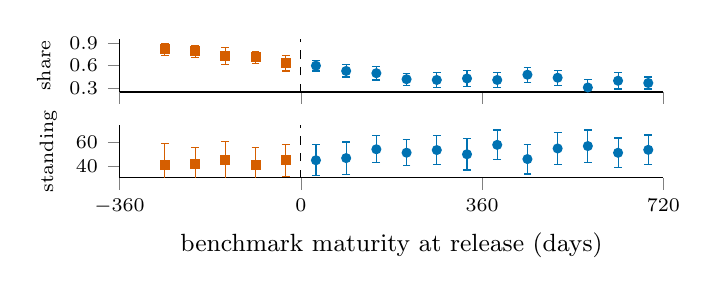
\begin{tikzpicture}
  \begin{axis}[causalre wide, height=2.25cm, xmin=-360, xmax=720, xtick={-360,0,360,720}, xticklabels={,,,}, ylabel={share}, ylabel style={font=\scriptsize}, ymin=0.25, ymax=0.95, ytick={0.3,0.6,0.9}, name=mech]
    \addplot[black, dashed, thin, forget plot] coordinates {(0,0.25) (0,0.95)};
    \addplot[cSF, only marks, mark=square*, mark size=1.4pt,
             error bars/.cd, y dir=both, y explicit]
      coordinates {(-270.000,0.82) +- (0,0.08) (-210.000,0.79) +- (0,0.08) (-150.000,0.73) +- (0,0.11) (-90.000,0.71) +- (0,0.08) (-30.000,0.63) +- (0,0.10)};
    \addplot[cNYC, only marks, mark=*, mark size=1.4pt,
             error bars/.cd, y dir=both, y explicit]
      coordinates {(30.000,0.60) +- (0,0.07) (90.000,0.53) +- (0,0.08) (150.000,0.50) +- (0,0.09) (210.000,0.42) +- (0,0.08) (270.000,0.41) +- (0,0.10) (330.000,0.43) +- (0,0.11) (390.000,0.41) +- (0,0.10) (450.000,0.48) +- (0,0.10) (510.000,0.44) +- (0,0.10) (570.000,0.31) +- (0,0.11) (630.000,0.40) +- (0,0.11) (690.000,0.37) +- (0,0.08)};
  \end{axis}
  \begin{axis}[causalre wide, height=2.25cm, xmin=-360, xmax=720, xtick={-360,0,360,720}, xlabel={benchmark maturity at release (days)}, ylabel={standing}, ylabel style={font=\scriptsize}, ymin=30, ymax=75, at={(mech.south west)}, anchor=north west, yshift=-12pt,
    legend to name=leg:boundary, legend columns=2]
    \addplot[black, dashed, thin, forget plot] coordinates {(0,30) (0,75)};
    \addplot[cSF, only marks, mark=square*, mark size=1.4pt,
             error bars/.cd, y dir=both, y explicit]
      coordinates {(-270.000,40.78) +- (0,18.37) (-210.000,41.55) +- (0,14.24) (-150.000,45.00) +- (0,16.04) (-90.000,41.36) +- (0,14.81) (-30.000,44.91) +- (0,13.75)};
    \addlegendentry{benchmark postdates the release}
    \addplot[cNYC, only marks, mark=*, mark size=1.4pt,
             error bars/.cd, y dir=both, y explicit]
      coordinates {(30.000,45.04) +- (0,13.16) (90.000,46.87) +- (0,13.81) (150.000,54.42) +- (0,11.65) (210.000,51.49) +- (0,11.25) (270.000,53.77) +- (0,12.19) (330.000,50.14) +- (0,13.47) (390.000,58.21) +- (0,12.71) (450.000,46.04) +- (0,12.76) (510.000,55.12) +- (0,13.60) (570.000,57.18) +- (0,13.73) (630.000,51.43) +- (0,12.65) (690.000,53.95) +- (0,12.64)};
    \addlegendentry{benchmark predates the release}
  \end{axis}
\end{tikzpicture}
\\[2pt]
{\footnotesize \ref{leg:boundary}}
% ---- end figures/fig_boundary ----
\caption{The mechanism and the outcome at the availability boundary. Top: the share of a
cell's window released after the focal model, against benchmark maturity at release;
it falls with maturity and jumps at the boundary. Bottom: within-benchmark standing
on the same axis, continuous through it. Sixty-day bins; intervals clustered on organisation.}
\label{fig:boundary}
\end{figure}

The share of a cell's window released after the focal model is 0.4683 for eligible cells and 0.7065 for placebo cells, against 0.5 for a two-sided window. Within release, the slope of standing on that share is $-30.63$ percentile points per unit among eligible cells alone. We plot standing versus the share of newer peers simultaneously for both types of cells in \autoref{fig:one-curve}. Instead of the two types of cells forming distinct point clouds, they follow a common downward trend that only appears after accounting for changes in the benchmark makeup (see \autoref{tab:decomposition}); eligible and placebo cells lie at different points on that line. By construction, eligible and placebo cells are separated and never overlap on their assignment variable, the maturity of the benchmark at release; thus the difference between eligible and placebo cells is obtained by extrapolation rather than comparison on the common support. As a robustness check, we probe the continuity of the regression at the cutoff, the only part of the assignment variable where the analysis is identified, see Section~\ref{sec:data-model} \citep{hahn2001identification}. The regression discontinuity analysis does not reveal a jump at the cutoff. Local linear regressions give negative coefficients for all bandwidths and orders, all confidence intervals include zero with the upper bound of the widest interval being $+8.05$, and the difference on a balance-driven bandwidth is $-2.52$ with a randomization $p$-value of 0.447 \citep{cattaneo2015randomization}. The two types of cells differ in mean maturity by 793 days, and the discrepancy between them is driven by that distance rather than the cutoff point itself (Appendix~\ref{sec:supporting} for the balance tests).

\begin{figure}[!htb]\centering
% ---- begin figures/fig_one_curve ----
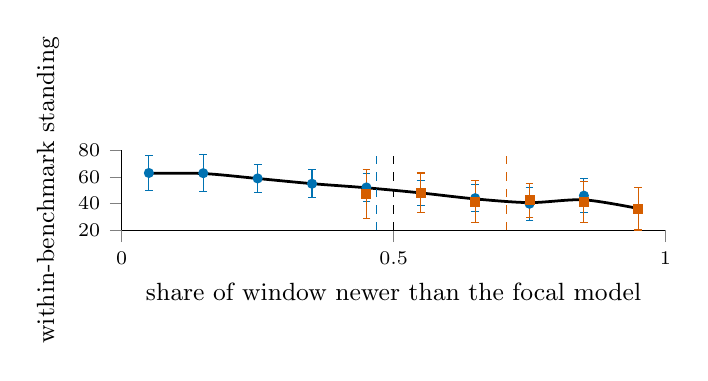
\begin{tikzpicture}
  \begin{axis}[causalre wide, height=2.6cm, xmin=0, xmax=1, xtick={0,0.5,1}, xlabel={share of window newer than the focal model}, ymin=20, ymax=80,
    ylabel={within-benchmark standing},
    legend to name=leg:onecurve, legend columns=3]
    \addplot[black, line width=1.0pt, smooth, forget plot]
      coordinates {(0.050,62.60) (0.150,62.49) (0.250,58.77) (0.350,54.92) (0.450,51.84) (0.550,47.99) (0.650,43.51) (0.750,40.74) (0.850,42.82) (0.950,36.33)};
    \addplot[black, dashed, thin, forget plot] coordinates {(0.5,20) (0.5,80)};
    \addplot[cNYC, dashed, thin, forget plot]
      coordinates {(0.468,20) (0.468,80)};
    \addplot[cSF, dashed, thin, forget plot]
      coordinates {(0.707,20) (0.707,80)};
    \addplot[cNYC, only marks, mark=*, mark size=1.4pt,
             error bars/.cd, y dir=both, y explicit]
      coordinates {(0.050,62.91) +- (0,13.17) (0.150,62.75) +- (0,13.73) (0.250,58.84) +- (0,10.53) (0.350,54.87) +- (0,10.42) (0.450,52.09) +- (0,10.63) (0.550,47.98) +- (0,9.26) (0.650,44.05) +- (0,9.94) (0.750,39.90) +- (0,12.27) (0.850,45.95) +- (0,12.64)};
    \addlegendentry{benchmark predates the release}
    \addplot[cSF, only marks, mark=square*, mark size=1.4pt,
             error bars/.cd, y dir=both, y explicit]
      coordinates {(0.450,47.28) +- (0,18.44) (0.550,48.08) +- (0,14.83) (0.650,41.55) +- (0,15.63) (0.750,42.43) +- (0,12.52) (0.850,41.34) +- (0,15.18) (0.950,36.23) +- (0,15.97)};
    \addlegendentry{benchmark postdates the release}
    \addplot[black, line width=1.0pt] coordinates {(0,0)};
    \addlegendentry{all cells pooled}
  \end{axis}
\end{tikzpicture}
\\[2pt]
{\footnotesize \ref{leg:onecurve}}
% ---- end figures/fig_one_curve ----
\caption{Standing against the share of a cell's window released after the focal model;
dashed verticals mark group mean shares, the black dashed line the symmetric 0.5. Eligible
and placebo cells lie on one declining curve, so the contrast between them is a position
on the curve, not a fact about disclosure. Intervals clustered on organisation.}
\label{fig:one-curve}
\end{figure}

It's possible to decompose standing as a weighted combination of percentile-ranks against older and newer peers with the share of newer peers as weight, $\text{percentile} = (1 - w)\,P_{\text{old}} + w\,P_{\text{new}}$ (exact cell-wise). The side-balanced standing, setting the weight to one half, available for 92.5\% of all cells (92.8\% for eligible-or-placebo cells), cuts the same slope to $-8.56$.

Despite the identity holding, the gradient is not a mere book-keeping tautology: permute the scores within the same benchmark, and the capability trend disappears while publishing dates, window membership, peer counts and newer shares are bit-wise identical. Under that null the slope has an average of $-0.09$ with a standard deviation of 3.12; the measured value of $-30.63$ is 9.8 standard deviations out, unmatched by any of the 300 draws. Further, fitting a linear regression within each benchmark of scores against publishing date, then reconstructing the scores as predicted values plus permuted residuals within each benchmark, meaning there's only a capability trend but no others, we are able to recover 93\% of the slope over 200 draws. The comparison-set geometry by itself is inert; it only introduces bias when combined with the existing trend in capabilities.

\subsection{Trimming and reweighting}\label{sec:core-recentring}

The phenomenon has a name in nonparametric estimation: local averages are biased near the edge of a support, and the standard remedies recentre rather than discard \citep{gasser1979,fan1992}. What is unusual is the boundary's coincidence with the endowment: a benchmark was available to a release exactly when the model did not sit at the left edge of that benchmark's coverage. The indicator of what a provider could have held is therefore the indicator of where the window is one-sided, and removing the edge removes the contrast. The coincidence has an older name, the age-period-cohort identity: release date, benchmark vintage and their difference are exactly collinear, and each has a measured signature here: $t_i$ in the capability trend, $\tau_b$ in saturation, $t_i - \tau_b$ in window composition. Only the linear components are unidentified in that structure \citep{fosse2019bounding,fosse2019review}, so what fails is a slope. Three sign restrictions bound it: capability rises with the calendar, later benchmarks are less saturated, and standing rises with maturity. All three are assumptions on unidentified components, each motivated by a measurement of an identified quantity. Under them the unidentified component accounts for at most 24 to 34\% of the placebo gap across specifications, roughly three percentile points, which is where the saturated regression also lands. The remainder is carried by the identified reduced-form slopes, and Appendix~\ref{sec:supporting} gives the derivation.

% ---- begin figures/table2_remedies ----
\begin{table}[!htb]
\centering
\small
\setlength{\tabcolsep}{4pt}
\begin{tabular}{lrrrrrr}
\toprule
Standing measure & Mean & Median & Positive & Sign-flip $p$ & Releases & Cells \\
\midrule
Windowed percentile, $\pm$182d & $+12.23$ & $+10.69$ & 78.1\% & 0.0001 & 146 & 100.0\% \\
Rank against all models ever & $+22.75$ & $+22.66$ & 89.0\% & 0.0001 & 146 & 100.0\% \\
Trim to two-sided windows & $+9.96$ & $+10.69$ & 72.2\% & 0.0001 & 115 & 70.4\% \\
Side-balanced percentile & $+9.14$ & $+9.62$ & 70.9\% & 0.0001 & 141 & 92.8\% \\
\bottomrule
\end{tabular}
\caption{%
The label-free placebo null under each candidate measure: release-level mean standing of eligible minus postdating benchmarks, in percentile points. Every entry should be zero. Sign-flip $p$ is the provider-clustered test of Section~\ref{sec:data-inference}; Cells, the share of cells carrying the measure.}
\label{tab:remedies}
\end{table}
% ---- end figures/table2_remedies ----

\autoref{tab:remedies} shows what follows. Ranking against every model ever scored nearly doubles the contamination; trimming to two-sided windows discards 30\% of the cells to remove 19\%, its row the uncorrected gap on the retained cells, composition rather than correction. Shortening the window does reduce the gap, to $+8.59$ at 91 days, but in proportion to the asymmetry it removes rather than by breaking the mechanism. Across four widths and four benchmark-count minima the gap is positive in
all 16 specifications, from $+8.59$ to $+21.66$, and tracks the eligible-minus-placebo gap in window composition at $r = 0.991$. Dropping any one of the 18 organisations leaves it between $+11.45$ and $+13.20$. The correction is a covariate, not a subsample.

One reading of that number would be too generous to it. Window composition is a function of the same dates that define the placebo indicator, so conditioning on it does not adjust for a confounder sitting outside the comparison; it splits the gap into the channel carrying it. A study that holds disclosure labels and wants an estimate of $\theta$ must first argue that window composition is settled before a provider decides what to report, or it conditions away part of what it measures. Provider identity explains little of the variance in window composition; Appendix~\ref{sec:supporting} reports the decomposition and the coverage tilt it does not correct.

The side-balanced percentile is the one change of measure doing substantial work, cutting the placebo mean to $+9.14$ and the eligible-cell gradient to $-8.56$. \autoref{fig:correction} in Appendix~\ref{sec:supporting} puts it against the uncorrected measure, near flat where cells are dense. Reweighting cannot reach what remains: balancing repairs the weight on each side of a model but not which models an evaluator chose to score early, so evaluator attention stays a confound. Undefined wherever a side is empty, it accompanies rather than replaces the uncorrected measure.
% ---- end sections/core ----
% ---- begin sections/external ----
\section{Evidence from HELM}\label{sec:external}

All of this has been on a percentile computed here, on a panel composed here. It is possible that only the percentile design has this property, and not leaderboards generally. For example, HELM Lite is a leaderboard that publishes all its accuracy data at each versioned release, and retains this history. It also publishes a pool-relative headline \citep{liang2022helm}, so the same evidence is read at 14 points in time while the pool expands.

When a leaderboard drifts, the first question is: has the suite changed? From v1.0.0 to v1.13.0, the 10 scenario columns are unchanged: no scenarios added, removed or renamed, except for a single column header relabel. Among the 24 models that span all 14 releases, all 240 published scenario scores remain bit-identical, as the evaluation pool expands from 30 to 91 models.

Published Mean win rate for all 24 constant models drifts (mean $|\text{drift}| = 0.1232$, max $|\text{drift}| = 0.2178$ for Mixtral 8x7B). This drift is mostly arithmetic: Mean win rate is computed as a win fraction, and a constant model compares against a larger, later pool over time; this drift correlates with initial standing ($r = -0.766$).

The key drift is in another direction. If the drift was a monotonic function of the bit-identical evidence then it would not change the ranking: monotonic transformations preserve rank order. This is not the case: 22 of the 24 constant models drift lower while two drift higher, and 5 of 276 pairs (1.8\%) reorder between the first and last version; all are published rank inversions under bit-identical evidence. \autoref{fig:helm}, in Appendix~\ref{sec:supporting}, plots the rank of each of the 24 constant models at the first version against the last. Each rank reversal is a crossing, visible and countable, on a bit-identical evidence base. This is distinct from overfitting to a test set \citep{roelofs2019meta}: here the evidence is bit-identical. It is the reference set that drifts. We observe a similar drift, from another cause, in \citet{singh2025leaderboard}: deprecation policy rather than a coverage boundary changing which models remain available; in both cases, the evidence remains constant and the ranking drifts with the reference set.

We also track a control: the HELM Capabilities leaderboard is from the same organisation, whose maintainers have diagnosed the win rate as pool-dependent \citep{xu2025capabilities}; it operates on the same infrastructure and release cadence, with a comparably expanding pool ($22 \to 68$ models in 16 versions). Instead of reporting the win fraction, its headline metric is an absolute mean over scenarios. Among 22 models that span all versions, all 110 scenario scores remain bit-identical, none of the 22 headline values drift, and there are no rank reversals, at the endpoints or at any time. Because the headline is an absolute mean over bit-identical scores on a fixed suite, it cannot drift with the pool: no drift is arithmetic, a scope condition rather than a test that could have failed.

None of this needs to be interpreted as a mistake on the part of HELM: their absolute headline, on their own Capabilities leaderboard, is the point. A pool-relative headline is a joint statement, about the model and about the population assessed beside it; read later as statements about the models alone, two such numbers move standing between providers for reasons belonging to neither. The problem of making different-time metrics comparable is a classical equating problem \citep{kolen2014}, which is bypassed by estimating a scale jointly \citep{epoch2026rosetta}. The panel and the leaderboard fail identically: the reference set, not the evidence, moves the number.
% ---- end sections/external ----
% ---- begin sections/reach ----
\section{Coding the Record}\label{sec:reach}

Possible reasons for absence from model cards include irrelevancy to the model, absence of running, or withholding after running. Of these only the latter qualifies as disclosure \citep{grossman1981,milgrom1981,dye1985}, and is thus one readers can price. The within-family drop narrows this: if the provider reported $b$ at $t$ but not at $t + 1$, and an independent score exists, then (i) $b$ is relevant, (ii) the provider had access to the benchmark harness, and (iii) the independent score serves as a registry-like counterfactual \citep{chan2004,dwan2013,kirkham2010}. But this does not establish that $b$ was run for $t + 1$, narrowing the \citet{dye1985} uncertainty but not closing it.

One coder coded the document released at release time for each of the 100 releases we can locate documents for (8 of 108 queued have none). We record which benchmarks they report, variants, mentions without scores, and explicitly-benign non-reports; we use these primitives and family history to mechanically derive the ORBIT categories. This results in 1,280 coded cells, 31 of which come from five of the most recent releases not in our pinned panel and are excluded. For a reliability study, a different coder double-coded a provider-stratified random fifth of the releases blind to the first and with no calibration communication (Appendix~\ref{sec:supporting} notes the one release where this blinding was broken). Kappa scores are for the derived cells \citep{cohen1960}, confidence intervals by resampling releases. We have agreement at 0.95 $[0.80, 1.00]$ on the primitive judgment of whether a benchmark was reported, at 0.85 $[0.72, 0.95]$ on the full set of categories, and at 0.81 $[0.48, 1.00]$ on the high vs.\ low suspicion categories. The E cell that each coder derives is identical; this is encouraging but too rare a category for a reliability estimate (Appendix~\ref{sec:supporting} gives the confusion structure). 76.9\% of the 1,249 eligible coded cells that resolve in our panel report no number, with release-level mean of 73.1\% $[65.9, 79.2]$. Note that this rate is descriptive, not yet evidence of selection.

% ---- begin figures/table3_coding ----
\begin{table}[!htb]
\centering
\small
\setlength{\tabcolsep}{5pt}
\begin{tabular}{lrrrr}
\toprule
Standing measure & Coded gap & 95\% CI & No labels & Difference \\
\midrule
Windowed percentile, $\pm$182d & $+11.40$ & $[+5.6, +17.0]$ & $+14.13$ & $-2.73$ \\
Side-balanced percentile, $\pm$182d & $+7.90$ & $[-0.4, +15.2]$ & $+9.82$ & $-1.92$ \\
Rank against all models ever & $+22.33$ & $[+18.0, +28.1]$ & $+24.50$ & $-2.17$ \\
Windowed percentile, $\pm$90d & $+8.15$ & $[+1.3, +14.7]$ & $+10.36$ & $-2.21$ \\
Windowed percentile, $\pm$365d & $+18.03$ & $[+13.9, +23.1]$ & $+20.53$ & $-2.50$ \\
\bottomrule
\end{tabular}
\caption{%
The coded omission deficit beside the label-free gap, percentile points, over 71 releases and 13 providers (70 side-balanced). No labels is the contrast with no disclosure coding; Difference is Coded gap minus No labels. Provider-clustered bootstrap intervals; four of five exclude zero.}
\label{tab:coding}
\end{table}
% ---- end figures/table3_coding ----

This section's result is \autoref{tab:coding}. The difference between disclosed and omitted is $+8.7$ points $[4.1, 13.9]$ across 63 releases, and the intended availability contrast between omitted eligible and post-dating cells is $+11.4$ $[5.6, 17.0]$ across 71 releases with both; the $p = 0.003$ would reject a zero null. When we read this against Section~\ref{sec:core}, we find that it is the availability gap: the label-free contrast on the same releases is $+14.1$, and the coded gap falls short by 1.9 to 2.7 points on every measure and window. This shortfall is an exact accounting identity: it is $+2.7$, the average over the same releases of the reported share $\times$ within-release reported-omitted gap, so our labels only change this contrast via composition.

And what's left is composition. The $+8.7$ points of standing between reported and omitted eligible benchmarks within release exceeds all 9,999 count-preserving random assignments ($p = 0.0001$, floored at the number of draws, null standard deviation 1.9), and cannot be generated by the availability gap. It's also robust to coding errors, variant reclassification, and leave-one-out analysis, because the availability gap is; and to benchmark identity: benchmark fixed effects alongside the release effects increase the coefficient from $+7.4$ to $+9.3$, and controlling for the window share leaves it at $+7.4$. But it cannot tell us that the standing caused the reporting: relevance, salience, within-eligible contamination all can move disclosure and performance together.

The remaining distance is possession; the original drop estimator and four possession cuts yield the same verdict. The drop estimator realises 16 drops across 15 releases and returns $+2.9$, opposite the withholding prediction, sign-flip $p = 0.25$ across five providers (the null its calibration priced). No document states that a benchmark was evaluated while reporting neither a score nor an outcome, across the 295 cells documenting a run. The change-based test (measuring each drop against its standing under the previous release) gives $-3.7$, the predicted sign, permutation $p = 0.16$ across 42 transitions; the possession tiers and equal-sized substitutions detect nothing further. Appendix~\ref{sec:supporting} gives detail, and three unrepaired limits: unlocatable documents, coverage that may follow provider emphasis, and best-across-scaffolds scoring.
% ---- end sections/reach ----
% ---- begin sections/conclusion ----
\section{Conclusion}\label{sec:conclusion}

We set out to measure how much of what could be reported goes unreported by choice. The coded record returns the number and the reason to distrust it: $+11.4$ points, rejecting zero yet short of its label-free counterpart by what composition implies, too imprecise to exclude a strategic component. Such a study turns composition into apparent concealment. Three claims separate: non-reporting is extensive, composition is performance-related, withholding not established, possession tests returning null, absent, or opposite-signed evidence. Dating instruments bounds the endowment, an access assumption, fixing where a model sits in a benchmark's coverage: what identifies it moves the measure pricing silence. A joint scale \citep{epoch2026rosetta} shrinks but does not close the placebo gap; a fixed suite carried across releases would make later silence informative, narrowing the \citet{dye1985} pooling and growing the 16-drop record.
% ---- end sections/conclusion ----

\bibliographystyle{plainnat}
\bibliography{refs}

\newpage
\appendix
% ---- begin sections/opportunity ----
\section{What a Provider Could Report}\label{sec:opportunity}

The comparisons above do not take into account that the set of results a provider could publish is increasing as new benchmarks are published. In our panel the number of dated benchmarks increases from 11 at the end of 2019 to 62 by 2026. Once a new benchmark appears it remains available to every release after it. In this sense, the number of possibilities is always weakly increasing.

At the same time, what a single release could report grows more slowly and less evenly. On average, by half-year, the number of eligible benchmarks per release is 6.8 in 2023 H1, declining to 3.9 in 2024 H1 as releases outpaced the instruments now used to score them, and it is 10.1 by 2026 H1. Thus, in our data, the two series move together over the sample and apart within it. This lends some evidence that the opportunity set may partially be shaped by the date of the releases and not by the providers.

This simple observation shows that a count of omissions is merely a count of the calendar. If reported tables do not expand one for one with the stock, then omission rates will increase by arithmetic forces alone, and comparisons between early and late releases are a comparison across eras, not across providers. All that remains is composition: which benchmarks providers drop, conditional on availability, compared to what an indifferent selection over the same set would have produced. To conduct this exercise it is necessary to know what was available. But once that is known it is also necessary to know how the release stood on each available benchmark. As we show in the rest of the paper, the latter is far more difficult than the former \citep{dranove2010}.
% ---- end sections/opportunity ----

% ---- begin sections/supporting ----
\section{Additional Checks}\label{sec:supporting}

\paragraph{Does the provider choose the window composition?}
Section~\ref{sec:core-recentring} conditions on window composition, which is admissible only if this is settled before the reporting decision. Fitting a regression of the fraction of a cell's window released after the focal model, on provider dummies, yields an $R^2$ of 0.071 (45 organisations); for comparison, fitting benchmark dummies yields $R^2$ of 0.002 (61 benchmarks), while the release date alone explains $R^2$ of 0.104. At the level of cells, window composition appears almost idiosyncratic. This is consistent with it being determined by the scoring schedule of the evaluator, as opposed to the provider. It is not enough to establish it.

\paragraph{Is the evaluator's coverage selective?}
The estimand also conditions on which cells are scored by the evaluator. This factor is by construction upstream of all others. On average, a release has 8.7 benchmarks scored; this varies with standard deviation 8.0, and spans a range of 1--38. It correlates with the provider's release count ($r = 0.203$) and with release date ($r = 0.265$), where releases from the densest quartile of providers average 9.6 scored benchmarks, versus 8.4 for the rest. This suggests a mild tilt toward larger and later providers, which we do not adjust for in this paper.

\paragraph{Bounding the unidentified component.}
Let $t$ be the release date, $\tau$ be the benchmark vintage, and $a = t - \tau$ be the maturity of the benchmark when the model met it. A regression of standing on these terms is by construction singular (the age-period-cohort problem), and only identifies $\Pi_p \equiv \beta_a + \beta_t$ and $\Pi_c \equiv \beta_\tau - \beta_a$, leaving a one-parameter family indexed by $\lambda \equiv \beta_a$. Fitting the reduced form across the 2,831 comparable cells, we obtain $\Pi_p = +4.12$ and $\Pi_c = -1.36$ percentile points per year. We can rely on three restrictions, derived from the body of the paper itself as opposed to external assumptions. (1) Capability is increasing in calendar time, i.e.\ $\beta_t \geq 0$. (2) Later benchmarks are less saturated, as directly quantified in Section~\ref{sec:core-boundary}, i.e.\ $\beta_\tau \leq 0$. (3) Standing is increasing in maturity, since a model on a young benchmark is ranked against newer peers, i.e.\ $\beta_a \geq 0$. Taken together, this means that $0 \leq \lambda \leq \min(\Pi_p, -\Pi_c) = 1.36$, where it is saturation, not capability, which is the binding restriction. On average, eligible and placebo cells differ by 2.17 years in maturity. Thus, at most, this unidentified component explains $1.36 \times 2.17 = 2.94$ percentile points, or 24\% of the observed gap. If we include centred squared and cubed terms in $t$ and $\tau$ (which are not collinear with $a$), then the ceiling moves to 34\% and 31\%. If we shuffle scores within benchmark, preserving every date and the rank deficiency while destroying the capability trend, then this quantity drops to an average of 0.02 percentile points across 30 draws, peaking at 0.24, confirming that the bound reflects the trend the geometry multiplies rather than the geometry alone.

\begin{figure}[H]\centering
% ---- begin figures/fig_helm ----
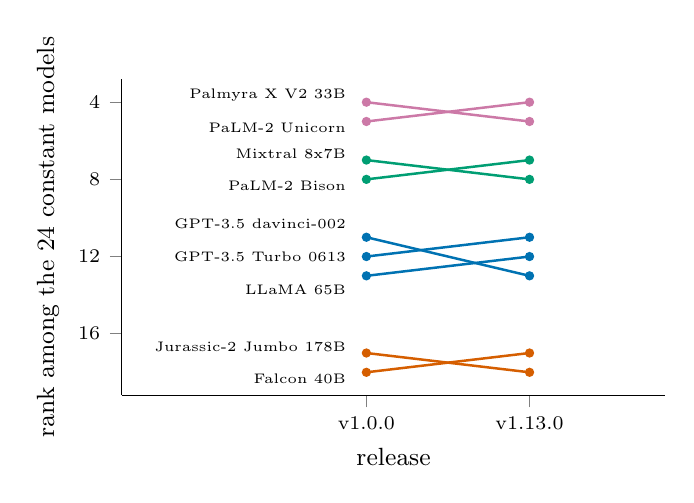
\begin{tikzpicture}
  \begin{axis}[causalre wide, height=5.6cm, y dir=reverse,
    xmin=0, xmax=1, ymin=2.8, ymax=19.2,
    xtick={0.45,0.75}, xticklabels={v1.0.0,v1.13.0}, xlabel={release},
    ytick={4,8,12,16}, ylabel={rank among the 24 constant models}]
    \addplot[cPNK, line width=0.9pt, mark=*, mark size=1.2pt, forget plot] coordinates {(0.45,4) (0.75,5)};
    \addplot[cPNK, line width=0.9pt, mark=*, mark size=1.2pt, forget plot] coordinates {(0.45,5) (0.75,4)};
    \addplot[cGRN, line width=0.9pt, mark=*, mark size=1.2pt, forget plot] coordinates {(0.45,7) (0.75,8)};
    \addplot[cGRN, line width=0.9pt, mark=*, mark size=1.2pt, forget plot] coordinates {(0.45,8) (0.75,7)};
    \addplot[cNYC, line width=0.9pt, mark=*, mark size=1.2pt, forget plot] coordinates {(0.45,11) (0.75,13)};
    \addplot[cNYC, line width=0.9pt, mark=*, mark size=1.2pt, forget plot] coordinates {(0.45,12) (0.75,11)};
    \addplot[cNYC, line width=0.9pt, mark=*, mark size=1.2pt, forget plot] coordinates {(0.45,13) (0.75,12)};
    \addplot[cSF, line width=0.9pt, mark=*, mark size=1.2pt, forget plot] coordinates {(0.45,17) (0.75,18)};
    \addplot[cSF, line width=0.9pt, mark=*, mark size=1.2pt, forget plot] coordinates {(0.45,18) (0.75,17)};
    \node[anchor=east, font=\tiny, text=black] at (axis cs:0.43,3.65) {Palmyra X V2 33B};
    \node[anchor=east, font=\tiny, text=black] at (axis cs:0.43,5.35) {PaLM-2 Unicorn};
    \node[anchor=east, font=\tiny, text=black] at (axis cs:0.43,6.65) {Mixtral 8x7B};
    \node[anchor=east, font=\tiny, text=black] at (axis cs:0.43,8.35) {PaLM-2 Bison};
    \node[anchor=east, font=\tiny, text=black] at (axis cs:0.43,10.30) {GPT-3.5 davinci-002};
    \node[anchor=east, font=\tiny, text=black] at (axis cs:0.43,12.00) {GPT-3.5 Turbo 0613};
    \node[anchor=east, font=\tiny, text=black] at (axis cs:0.43,13.70) {LLaMA 65B};
    \node[anchor=east, font=\tiny, text=black] at (axis cs:0.43,16.65) {Jurassic-2 Jumbo 178B};
    \node[anchor=east, font=\tiny, text=black] at (axis cs:0.43,18.35) {Falcon 40B};
  \end{axis}
\end{tikzpicture}
% ---- end figures/fig_helm ----
\caption{The nine HELM Lite models whose published order changed between the first release
and the last, ranked among the 24 whose 240 scenario scores are bit-identical throughout;
coloured by group of mutually reversing models, four groups and five reversed pairs in all. The control: across 16 HELM Capabilities releases behind an
absolute headline, with the pool growing from 22 to 68, none of the 22 constant models'
headline values moved and no pair reversed.}
\label{fig:helm}
\end{figure}

\paragraph{The cutoff is a discontinuity.}
Treatment eligibility $\mathbf{1}[t_i > \tau_b]$, being a deterministic function of dates, is the problem that global approaches confront. Equating across different instruments requires a common conditional relation across samples, which samples split by a cutoff do not satisfy \citep{sinharay2010missing}; weighting by observed cell probability assumes a non-vanishing observed probability, which a deterministic cutoff rules out \citep{ma2019missing}; finally, a deterministic cutoff is a sharp discontinuity so that, at the cutoff, standing is identified under continuity conditions regardless of what is true elsewhere \citep{hahn2001identification}. We estimate local linear regressions using a triangular kernel and errors clustered at the provider level with results of $-8.82$ (4.76) at $\pm 60$ days, $-6.85$ (4.09) at $\pm 90$, $-4.08$ (3.11) at $\pm 180$ and $-2.85$ (2.35) at $\pm 250$; adding a quadratic term at each bandwidth does not take any of these estimates across zero. All eight estimates are negative; every confidence interval includes zero and the highest upper limit of the CI is $+8.05$, strictly below the $+12.23$ the global comparison reports. Consistent with local randomization inference at the cutoff \citep{cattaneo2015randomization}, we also increase symmetric bandwidths around the cutoff and evaluate balance of the release's benchmark count, scaffold count, and scaffold spread; the minimum $p$ value over these tests is 0.335 at $\pm 20$ days and 0.571 at $\pm 40$, decreasing to 0.058 at $\pm 60$; we pick $\pm 40$ days, ad hoc based on the balance tests, and thus the randomization $p$ value reported below is not corrected for that choice. The same difference is $-5.96$ ($p = 0.23$) at $\pm 20$ days and $+0.43$ ($p = 0.88$) at $\pm 60$. With 113 postdating and 114 eligible cells in this range, the difference in mean standing is $-2.52$, randomization $p$ of 0.447. There is no bunching against the cutoff: the ratio of cell counts within 30 days after vs.\ 30 days before the cutoff is 0.95 (80 vs.\ 84 cells) \citep{mccrary2008manipulation}. The mechanism is discontinuous where standing is not. At the cutoff, the fraction of a cell's window released after the focal model has a step size of $+0.083$, translating, using the $-30.63$ gradient for eligible cells, to about $-2.5$ percentile points, comfortably within all confidence intervals above, so the cutoff design discriminates concealment from the availability gap only above that size at the cutoff; at the narrowest bandwidths, the full $-12.23$ is not rejected either. Peer count and raw score are continuous. The global difference arises because the average cell maturity differs between the two samples by 793 days, not from anything at the cutoff.

\paragraph{A standing measure with no comparison window.}
The conclusion points at a scale estimated jointly across benchmarks rather than against
contemporaries, which removes the comparison window from the measure entirely. Fitting one does not
remove the gap. Ability and difficulty are estimated together over the 63 benchmarks reported on a
common zero-to-one scale, on a logit link, with the loading ridged toward one because a free loading
is unidentified at this density and takes slopes past $65{,}000$. Restricting to benchmarks carrying
at least twenty releases and releases carrying at least three benchmarks leaves 1,669 eligible cells
over 31 benchmarks. The model is fit on eligible cells alone, so the 226 postdating cells it can
score are out of sample.

The eligible-minus-placebo gap in the residuals is $+0.336$ residual standard deviations, against
$+0.449$ for the windowed percentile on the same contrast, positive in 64.0\% of the 89 releases
holding both kinds, at $p = 0.005$. Removing the window shrinks the gap by about a quarter and
leaves it positive, which puts a jointly estimated scale beside trimming at 19\% and side-balancing at 25\%, each on its own scale,
rather than ahead of them. Its difficulty parameters are estimated from the maturity-selected cells that exist, so part of the surviving gap may be the same selection re-expressed, and its placebo cells are scored out of sample while every eligible cell is in sample, an asymmetry the contrast inherits. Shuffling scores within benchmark, which leaves every date and the rank
deficiency untouched, drops the same quantity to 0.02 on average over 30 draws.

\begin{figure}[H]\centering
% ---- begin figures/fig_correction ----
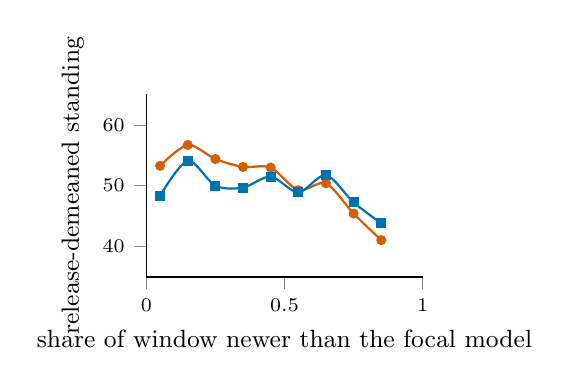
\begin{tikzpicture}
  \begin{axis}[causalre body, xmin=0, xmax=1, xtick={0,0.5,1}, xlabel={share of window newer than the focal model}, ymin=35, ymax=65,
    ylabel={release-demeaned standing},
    legend to name=leg:correction, legend columns=2]
    \addplot[cSF, smooth, mark=*, mark size=1.4pt]
      coordinates {(0.050,53.27) (0.150,56.70) (0.250,54.39) (0.350,53.09) (0.450,52.98) (0.550,49.26) (0.650,50.38) (0.750,45.42) (0.850,41.06)};
    \addlegendentry{windowed percentile}
    \addplot[cNYC, smooth, mark=square*, mark size=1.4pt]
      coordinates {(0.050,48.37) (0.150,54.10) (0.250,50.00) (0.350,49.69) (0.450,51.49) (0.550,48.90) (0.650,51.74) (0.750,47.26) (0.850,43.81)};
    \addlegendentry{side-balanced}
  \end{axis}
\end{tikzpicture}
\\[2pt]
{\footnotesize \ref{leg:correction}}
% ---- end figures/fig_correction ----
\caption{The side-balanced percentile against the windowed one, on eligible cells within release.
The windowed measure slopes across the range while the side-balanced one is close to flat where cells are dense; the quoted gradients, $-30.63$ to $-8.56$ per unit share, are the within-release regression slopes on these cells, and the release-demeaned binned means shown are correspondingly flatter.}
\label{fig:correction}
\end{figure}

A backward-only standing, position among older peers alone, removes the window's forward half entirely and leaves the label-free contrast at $+12.11$ across 142 releases, so the gap does not come from look-ahead.

\paragraph{Drop-design ceiling and calibration.}
The panel contains 144 adjacent same-family release pairs covering 711 shared eligible benchmarks and 15 organisations. Requiring both releases in a pair to carry at least eight scored benchmarks leaves 37 pairs, 482 shared benchmarks, and 8 organisations, the effective cluster count, in the regime where Section~\ref{sec:data-inference} reports no analytic standard error. Under the null of no selective withholding, the sampling standard deviation of a drop gap, over 400 draws for each of 117 qualifying releases, is 19.4 percentile points when one benchmark is dropped, 14.4 when two are and 12.4 when three are. At conventional two-sided size a single-drop event must therefore move the gap by roughly 38 points before it separates from noise, three times the contamination itself, and no single drop can be read alone.

\paragraph{Possession evidence.}
Selective withholding is a statement about results a provider held and did not print, and the disclosure label observes only the printing. Four cuts organise how far the record reaches toward possession. The direct cases first: no document explicitly states that a benchmark was evaluated while reporting neither a score nor an outcome, so the direct-withholding category is empty over the 295 cells where a run is documented; the six named-without-number cells all carry an outcome in a figure, a chart, or a comparative claim. Second, the omission deficit stratified by evidence tier. Withholding predicts the deficit weakens, and eventually inverts, as possession evidence strengthens; composition predicts no gradient. The point estimates are $+18.9$ over 21 releases for dropped benchmarks, $+11.3$ over 51 for peer-reported omissions, and $+11.3$ over 69 for silent ones. The deficit does not become more negative as possession evidence strengthens; the dropped tier instead carries the largest positive deficit, a gradient that does not match the signature withholding predicts. Third, a change-based drop test. The estimator above compares levels; a sharper question is whether a benchmark is dropped after the family's standing on it deteriorates, which differences out persistent salience and relevance. Over the 42 family transitions with a scored predecessor report, 33 dropped and 86 retained cells give a dropped-minus-retained change of $-3.7$ percentile points, the sign withholding predicts, at a count-preserving permutation $p = 0.16$ within transitions; on raw scores, kept where both sit on the unit interval, the gap is $-0.7$ points at $p = 0.71$. Both samples cut the 63 derived drop cells: the level estimator keeps the 16 sitting in releases that also retain at least two reported benchmarks to compare against, while the change-based test keeps the 33 with an independent score under both predecessor and successor and imposes no retention floor. Fourth, substitutions. Requiring the reporting table to hold its size while one benchmark is dropped and another inserted, the case a fixed-table explanation cannot cover, leaves no qualifying case in the record. Nothing in the four detects withholding. The change-based gap is directionally consistent with it and statistically indistinguishable from its permutation null; every other cut is null, absent, or opposite in sign.

\paragraph{Reliability detail.}
The second coding covers 20 of the 100 readable releases, drawn stratified by provider.
Derived categories import contemporaries' evidence across releases, a dependence the release resampling does not model. Across 15 of them, 194 derived cells pair: one drawn release is a zero-disclosure document whose blank evidence rows the pairing drops, a conservative exclusion since all
eleven of its cells are trivial agreements, and four drawn releases sit outside the pinned
panel. The reported-versus-not cross-tabulation is one-directional, 47 jointly reported and 143
jointly not: no cell the first coder called reported was coded otherwise by the second, and
the four reversals all sit on one release whose second-coding note records retaining four
contested scores despite the first coder's disagreement, an exposure that breaks blindness
for that release. Excluding it, reported-versus-not agreement is exact and the
full-category $\kappa$ is 0.88 on 182 cells. Of the 14 disagreements overall, seven are
the variant boundary between C and A, one a bare mention against a value, two the derived
split between G and H on a single release, and four the exposed release above.
Three limits of the record are candidly unrepaired: the eight releases without a locatable
document are unlikely to be missing at random and plausibly document less; the evaluator's
coverage may itself respond to what providers emphasise, which would tilt the reported set
upward by sampling; and the best-across-scaffolds score rule is not probed for asymmetry
across the boundary. High-suspicion marginals match exactly at 5.7\% for each coder, which is why the split
$\kappa$ holds at 0.81 despite the category's rarity; its wide interval reflects eleven such
cells concentrating in a few releases.

\paragraph{Provider-only clustering, for comparison.}
The manuscript's regressions cluster on provider and benchmark jointly. Provider-only errors are
consistently smaller: 1.271 against 2.038 on the release-effects row, a ratio of 1.60, and 1.652
against 1.748 on the fully saturated row, a ratio of 1.06. The benchmark dimension carries real
dependence on the raw contrast and almost none once benchmark effects and the window terms are in,
which is what the decomposition says it should. The headline sign-flip test at $p = 0.0001$
preserves provider dependence only; the two-way regression row above is the statement that the
contamination survives both dimensions, at $t = -6.6$.
% ---- end sections/supporting ----

\newpage
% ---- begin sections/checklist ----
\section*{NeurIPS Paper Checklist}

\begin{enumerate}

\item {\bf Claims}
    \item[] Question: Do the main claims made in the abstract and introduction accurately reflect the paper's contributions and scope?
    \item[] Answer: \answerYes{}
    \item[] Justification: The abstract and introduction state both findings within their identified scope: the coded omission gap is indistinguishable from the label-free gap, and within-release composition tracks standing. Section~\ref{sec:reach} reports the reliability of the coding behind them.


\item {\bf Limitations}
    \item[] Question: Does the paper discuss the limitations of the work performed by the authors?
    \item[] Answer: \answerYes{}
    \item[] Justification: Limitations appear where they bear on the argument rather than only at the end. Section~\ref{sec:data-model} bounds the estimand and states that the reported omission rate is descriptive and identifies no withholding; Section~\ref{sec:core-boundary} states that the conditioning is a decomposition rather than a control strategy, and what a study holding disclosure labels would additionally have to argue; Section~\ref{sec:core-recentring} reports the corrections that fail and the coverage the balanced measure loses; Section~\ref{sec:reach} reports the ceiling on the design that narrows endowment uncertainty furthest, its 16 realised drops, and the underpowered null they return.


\item {\bf Theory assumptions and proofs}
    \item[] Question: For each theoretical result, does the paper provide the full set of assumptions and a complete (and correct) proof?
    \item[] Answer: \answerYes{}
    \item[] Justification: Section~\ref{sec:data-model} states one identification result, that a temporal eligibility gate cannot satisfy the exclusion restriction the design needs, and gives its argument in full: the three date variables are exactly collinear, so excluding one requires that at least two of them not move standing. Section~\ref{sec:core} shows all three move it. Appendix~\ref{sec:supporting} states the three sign restrictions used to bound the unidentified component and derives the bound from them. Everything else in Section~\ref{sec:data-model} restates published results with citation.


    \item {\bf Experimental result reproducibility}
    \item[] Question: Does the paper fully disclose all the information needed to reproduce the main experimental results of the paper to the extent that it affects the main claims and/or conclusions of the paper (regardless of whether the code and data are provided or not)?
    \item[] Answer: \answerYes{}
    \item[] Justification: Every number in the paper is written by one command into a single machine-readable file, and the data snapshot it was computed against is pinned by a per-file SHA-256 manifest in the released code. Section~\ref{sec:data} states the release key, the eligibility rule, the window width, and which estimates impose a minimum benchmark count and which do not.



\item {\bf Open access to data and code}
    \item[] Question: Does the paper provide open access to the data and code, with sufficient instructions to faithfully reproduce the main experimental results, as described in supplemental material?
    \item[] Answer: \answerYes{}
    \item[] Justification: Code and derived data are released with instructions. The independent scores are redistributed by their publisher under CC-BY and are fetched rather than copied, then verified against the pinned manifest, so an upstream change is reported rather than silently absorbed. The external leaderboard evidence is frozen with a SHA-256 per source file, because a public leaderboard moves and the argument depends on the exact values.



\item {\bf Experimental setting/details}
    \item[] Question: Does the paper specify all the training and test details (e.g., data splits, hyperparameters, how they were chosen, type of optimizer) necessary to understand the results?
    \item[] Answer: \answerYes{}
    \item[] Justification: There is no model training. The choices that affect the estimates are stated in Section~\ref{sec:data}: the release key, the rule for collapsing scaffold variants, the 182-day comparison window, which estimates impose a minimum benchmark count and which do not, and the treatment of pairs whose benchmark vintage is unverified.


\item {\bf Experiment statistical significance}
    \item[] Question: Does the paper report error bars suitably and correctly defined or other appropriate information about the statistical significance of the experiments?
    \item[] Answer: \answerYes{}
    \item[] Justification: Section~\ref{sec:data-inference} states the inference protocol. The cluster count is small and unevenly distributed, so below twelve clusters no analytic standard error is reported, coefficients in that range use a restricted wild cluster bootstrap, release-level means use a cluster sign-flip randomization test, and no result is called significant on a cluster-t alone. Table~1 reports a standard error with every coefficient, the headline contrast carries a randomization p-value, and the permutation null is reported with its mean, its spread and the number of draws reaching the observed value.


\item {\bf Experiments compute resources}
    \item[] Question: For each experiment, does the paper provide sufficient information on the computer resources (type of compute workers, memory, time of execution) needed to reproduce the experiments?
    \item[] Answer: \answerYes{}
    \item[] Justification: All analysis runs in seconds on a laptop. There is no training, no accelerator use, and no discarded run.


\item {\bf Code of ethics}
    \item[] Question: Does the research conducted in the paper conform, in every respect, with the NeurIPS Code of Ethics \url{https://neurips.cc/public/EthicsGuidelines}?
    \item[] Answer: \answerYes{}
    \item[] Justification: The work uses published benchmark scores and public release documents, involves no human subjects and no personal data, and makes no claim about any individual.



\item {\bf Broader impacts}
    \item[] Question: Does the paper discuss both potential positive societal impacts and negative societal impacts of the work performed?
    \item[] Answer: \answerYes{}
    \item[] Justification: Section~\ref{sec:external} states the consequence for a reader of a pool-relative leaderboard, namely that such a number describes standing within one vintage of the evaluated pool rather than a property of the model. The conclusion states that whether the record needed to measure withholding should grow is a reporting-standard question. The paper does not attribute concealment to any named provider, because the design does not support that.


\item {\bf Safeguards}
    \item[] Question: Does the paper describe safeguards that have been put in place for responsible release of data or models that have a high risk for misuse (e.g., pre-trained language models, image generators, or scraped datasets)?
    \item[] Answer: \answerNA{}
    \item[] Justification: No model, dataset or other asset with misuse potential is released. The release is analysis code and derived tables built from already public sources.


\item {\bf Licenses for existing assets}
    \item[] Question: Are the creators or original owners of assets (e.g., code, data, models), used in the paper, properly credited and are the license and terms of use explicitly mentioned and properly respected?
    \item[] Answer: \answerYes{}
    \item[] Justification: The independent scores are credited to their publisher and used under CC-BY, and the external leaderboard is cited to its published description. Both are named in the text and in the released code.


\item {\bf New assets}
    \item[] Question: Are new assets introduced in the paper well documented and is the documentation provided alongside the assets?
    \item[] Answer: \answerYes{}
    \item[] Justification: The released code documents how each number is produced, the snapshot manifest records the exact data build, and the frozen external evidence records a source URL, a retrieval date and a SHA-256 for every file.


\item {\bf Crowdsourcing and research with human subjects}
    \item[] Question: For crowdsourcing experiments and research with human subjects, does the paper include the full text of instructions given to participants and screenshots, if applicable, as well as details about compensation (if any)?
    \item[] Answer: \answerNA{}
    \item[] Justification: The work involves no crowdsourcing and no human subjects.


\item {\bf Institutional review board (IRB) approvals or equivalent for research with human subjects}
    \item[] Question: Does the paper describe potential risks incurred by study participants, whether such risks were disclosed to the subjects, and whether Institutional Review Board (IRB) approvals (or an equivalent approval/review based on the requirements of your country or institution) were obtained?
    \item[] Answer: \answerNA{}
    \item[] Justification: The work involves no human subjects, so no review board approval was required.


\item {\bf Declaration of LLM usage}
    \item[] Question: Does the paper describe the usage of LLMs if it is an important, original, or non-standard component of the core methods in this research? Note that if the LLM is used only for writing, editing, or formatting purposes and does \emph{not} impact the core methodology, scientific rigor, or originality of the research, declaration is not required.
    %this research?
    \item[] Answer: \answerYes{}
    \item[] Justification: All disclosure-coding categories standing in the paper were hand-assigned by a human coder from archived release-time documents under the frozen protocol, with an independent second coder recoding a provider-stratified 20\% sample (Section~\ref{sec:reach}), so no number reported here depends on a model's judgment. A superseded early pass had used a large language model on the same task; those labels were cleared before analysis and none enters. Every number is produced by the released code from the pinned snapshot. Language models were otherwise used only for writing and code assistance.


\end{enumerate}
% ---- end sections/checklist ----

\end{document}
